\subsection{Experimental Evaluation}
\label{comesh:sec:expts}
We present: 
(i) Raspberry Pi Lab Deployments   (\Cref{comesh:sec:pidep}) driven by mini-maps of a smart building and a smart farm, 
(ii) Large-scale Simulations  (\Cref{comesh:sec:simres}), \&  
(iii) Map-based Simulations with real Routine workloads (\Cref{comesh:sec:mapsim}). 


\subsubsection{Raspberry Pi Deployments}
\label{comesh:sec:pidep}

We implemented \sysname{} in  Raspberry Pi (RPi) 4, via  {12.9K lines of Java code}. Our deployments use commercial RPi 4 model B,
with 2GB of LPDDR4 RAM, Broadcom BCM2711 quad-core CPU of 1.5GHz Cortex-A72 cores, and communicating via WiFi.
To implement the central approach, we use an additional 17$^{th}$ Pi device as the central hub. 
To create the mesh topology, we attenuate RPi's strong signal by consistently wrapping each device in aluminum foil to lower transmission power to 15dBm~\cite{Safehome}.
We use OLSR routing~\cite{olsrd} as it is standard in Pi 4s.
For membership, we use Medley~\cite{medley}.

\sysname{} is configured to use \kgroups{} with expected $k=3$ smart devices per \kgroup, and a device \kgroup{} monitors its devices every second. The default locking is  SLA locking (\Cref{comesh:subsubsec:sla}).
To avoid cold start biases, we start measurements 10 s after \sysname{} is initialized. Each data point involves at least 5 trial runs with different seeds.
Epoch length is 60 s.

\noindent{\bf Routine workload.} Multiple routines may be triggered independently and simultaneously; the same routine is never re-triggered within 10 s of its own previous invocation. For each routine, its number of triggering (resp. actuated) devices is drawn from a Gaussian distribution ranging from a low of 2 (resp. 1) to a high of $N/4$, with a mean of 2 and a standard deviation of 1; triggering and actuated devices are then chosen uniformly at random. We inject new device-state events uniformly every $[0.5, 1]$ s. \Cref{comesh:fig:rtn_iat} shows the CDF of the resulting routine inter-arrival times for each of our device counts ($N = 4, 16, 64, 144$).

\begin{figure}[tb!]
    \centering
    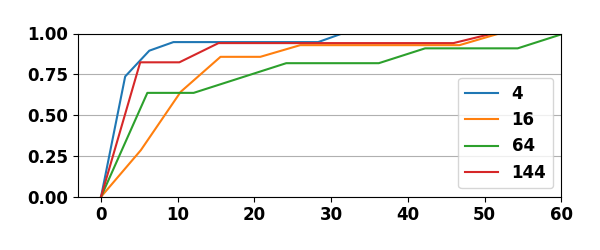
\includegraphics[width=0.55\linewidth,alt={CDF plot of routine inter-arrival times. x-axis: inter-arrival time in seconds (0 to 60); y-axis: cumulative probability (0 to 1). Four step curves, one per device count (4, 16, 64, and 144 devices). All curves rise steeply within the first 10 to 20 seconds and approach 1.0, with the 64-device curve having the longest tail (reaching 1.0 only near 50 seconds) and the smaller device counts concentrating most inter-arrivals below about 15 seconds.}]{CoMesh/figures/exp_eval/rtns_r20_iat_cdf.png}
    \caption{\bf \small Deployment: CDF of routine inter-arrival times (seconds) for different device counts. {\it $N = 4, 16, 64, 144$}.}
    \medskip
    \label{comesh:fig:rtn_iat}
\end{figure}

\begin{figure}[tb!]
    \centering
    \begin{subfigure}[b]{0.35\linewidth}
        \centering
        \includegraphics[width=\textwidth, angle = 270, origin=c,alt={Photograph of the Raspberry Pi testbed arranged in a line topology, representing the Mini \Bldg{} (\Mob) deployment.}]{CoMesh/figures/exp_eval/rpi_line_topo.JPG}
        \caption{\small Mini \Bldg{} (\Mob). From \Cref{comesh:fig:smart-building}.}
        \label{comesh:subfig:line_topo}
    \end{subfigure}
    \hspace{5pt}
    \begin{subfigure}[b]{0.35\linewidth}
        \centering
        \includegraphics[width=\textwidth,alt={Photograph of the Raspberry Pi testbed arranged in a grid topology, representing the Mini \Grid{} (\Minigrid) deployment.}]{CoMesh/figures/exp_eval/rpi_grid_topo.JPG}
        \caption{\small Mini \Grid{} (\Minigrid). From \Cref{comesh:fig:smart-farm}.}
        \label{comesh:subfig:grid_topo}
    \end{subfigure}
    \par\medskip
    \begin{subfigure}[b]{0.35\linewidth}
        \centering
        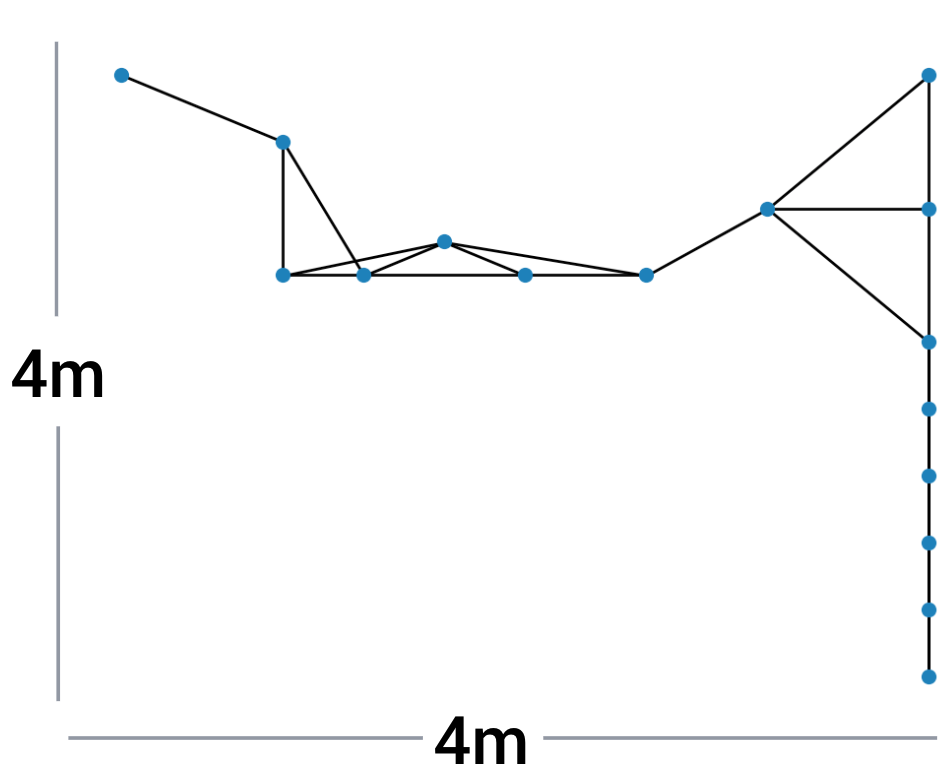
\includegraphics[width=0.78\textwidth,alt={Schematic of the measured node placement and inter-node link distances for the Raspberry Pi deployment's Mini \Bldg{} (\Mob) topology.}]{CoMesh/figures/exp_eval/l_topo_measurements.png}
        \caption{\small Mini \Bldg{} (\Mob). From \Cref{comesh:fig:smart-building}.}
        \label{comesh:subfig:line-topo-graph}
    \end{subfigure}
    \hspace{5pt}
    \begin{subfigure}[b]{0.35\linewidth}
        \centering
        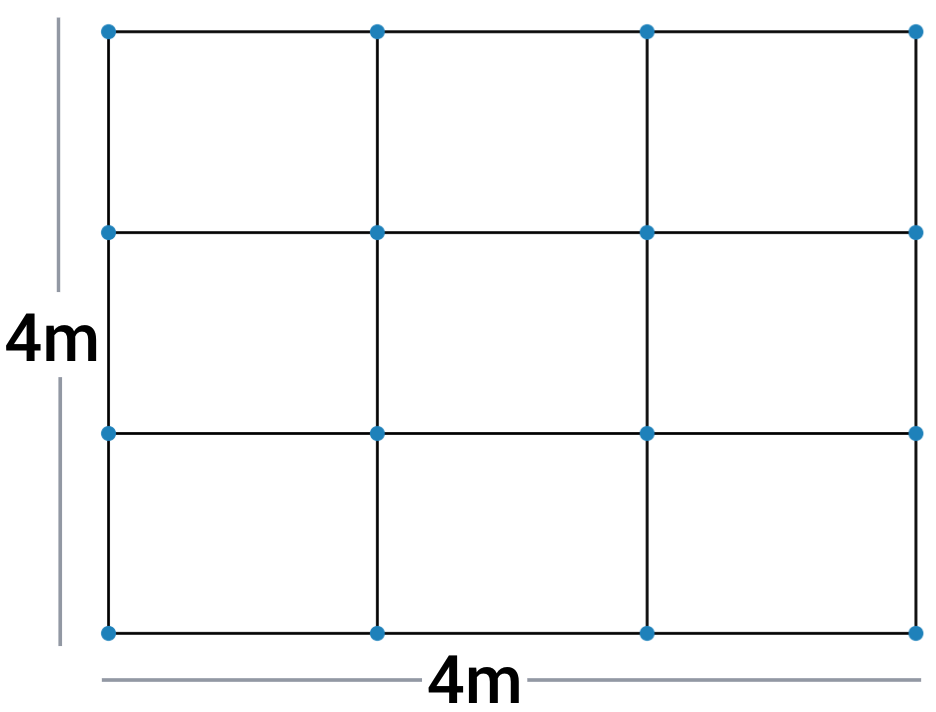
\includegraphics[width=0.78\textwidth,alt={Schematic of the measured node placement and inter-node link distances for the Raspberry Pi deployment's Mini \Grid{} (\Minigrid) topology.}]{CoMesh/figures/exp_eval/grid_topo_measurements.png}
        \caption{\small Mini \Grid{} (\Minigrid). From \Cref{comesh:fig:smart-farm}.}
        \label{comesh:subfig:grid-topo-graph}
    \end{subfigure}
    \caption{\bf \small Deployment: Raspberry Pi Topologies. {\it From \Cref{comesh:fig:smart-building,comesh:fig:smart-farm}.}}
    \medskip
    \label{comesh:fig:rpi_topos}
\end{figure}

We implement the two Pi topologies shown in \Cref{comesh:fig:rpi_topos}, based on  \Cref{comesh:fig:smart-building,comesh:fig:smart-farm}. They are: 
(i) a {\it Mini \Bldg{}}  topology ({\it \Mob} in plots), based on the L-shaped map of the  \Bldg{}   from \Cref{comesh:fig:smart-building}; and (ii) a {\it Mini \Grid{} topology} ({\it \Minigrid} in plots) based on \Cref{comesh:fig:smart-farm}, modeled via a 
4 $\times$ 4 2D {Grid}. Each covers an area of 4 meters $\times$ 4 meters. 
Note the \Mob{} topology's diameter (in hops) is higher than \Minigrid's. 

\begin{figure}[tb!]
    \centering
    \begin{minipage}[b]{0.48\textwidth}
        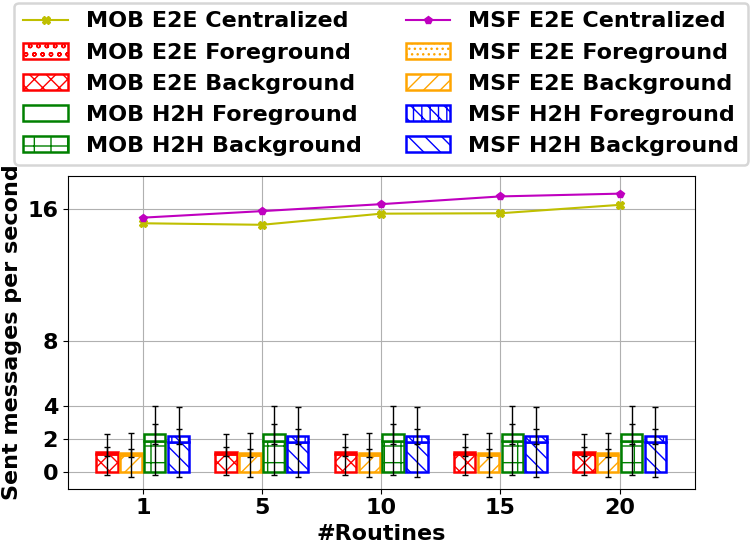
\includegraphics[width=\textwidth,alt={Line-and-bar chart. x-axis: number of routines (1, 5, 10, 15, 20); y-axis: sent messages per second on a log scale (1 to 16). The two centralized end-to-end lines (Mini \Bldg{} and Mini \Grid{}) sit near 16 messages per second and stay roughly flat as routines increase, while all of \sysname{}'s bars (end-to-end and hop-to-hop, foreground and background, for both deployments) stay low between about 1 and 2 messages per second and also flat, roughly an order of magnitude below the centralized lines.}]{CoMesh/figures/exp_eval/bandwidth_xrtn.png}
        \caption{\bf \small  Deployment:  Centralized (lines) vs. \sysname{} (bars): Bandwidth.  {\it \Mob{} = Mini \Bldg, \MSF{} = Mini \Grid.}
        }
        \medskip
        \label{comesh:fig:bw_centralized_skytali}
    \end{minipage}
    \hfill
    \begin{minipage}[b]{0.46\textwidth}
        \centering
        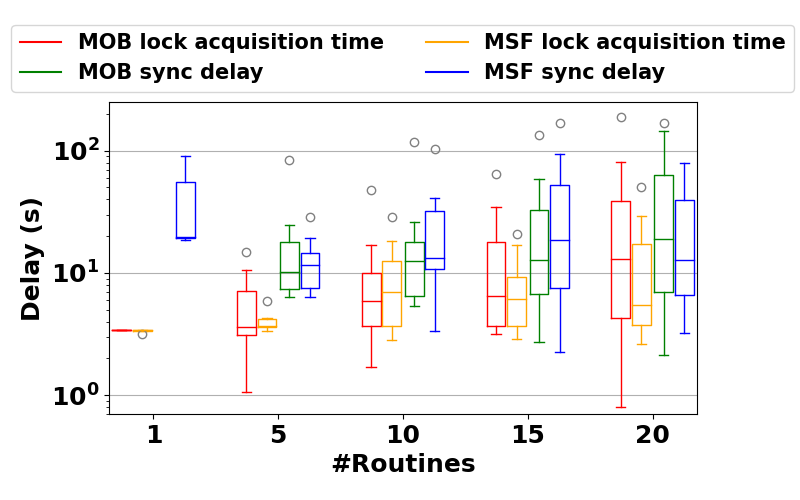
\includegraphics[width=1.02\textwidth,alt={Grouped box-and-whisker plot. x-axis: number of routines (1, 5, 10, 15, 20); y-axis: delay in seconds on a log scale (about 1 to over 100). Four series per group: Mini \Bldg{} and Mini \Grid{} lock-acquisition time, and Mini \Bldg{} and Mini \Grid{} sync delay. Medians are stable and sit roughly between 3 and 20 seconds, and the spread and outliers grow with more routines, with some outliers reaching about 100 to 200 seconds at 15 to 20 routines.}]{CoMesh/figures/exp_eval/client_sync_delay_xrtn.png}
        \caption{\bf \small Deployment: Lock Acquisition Time and Sync Delay. {\it \Mob{} = Mini \Bldg, \MSF{} = Mini \Grid.}
        }
        \medskip
        \label{comesh:fig:la_sync_mul_rtns}
    \end{minipage}
\end{figure}

\begin{figure}[ht]
    \centering
    \begin{minipage}[b]{0.52\textwidth}
        \centering
        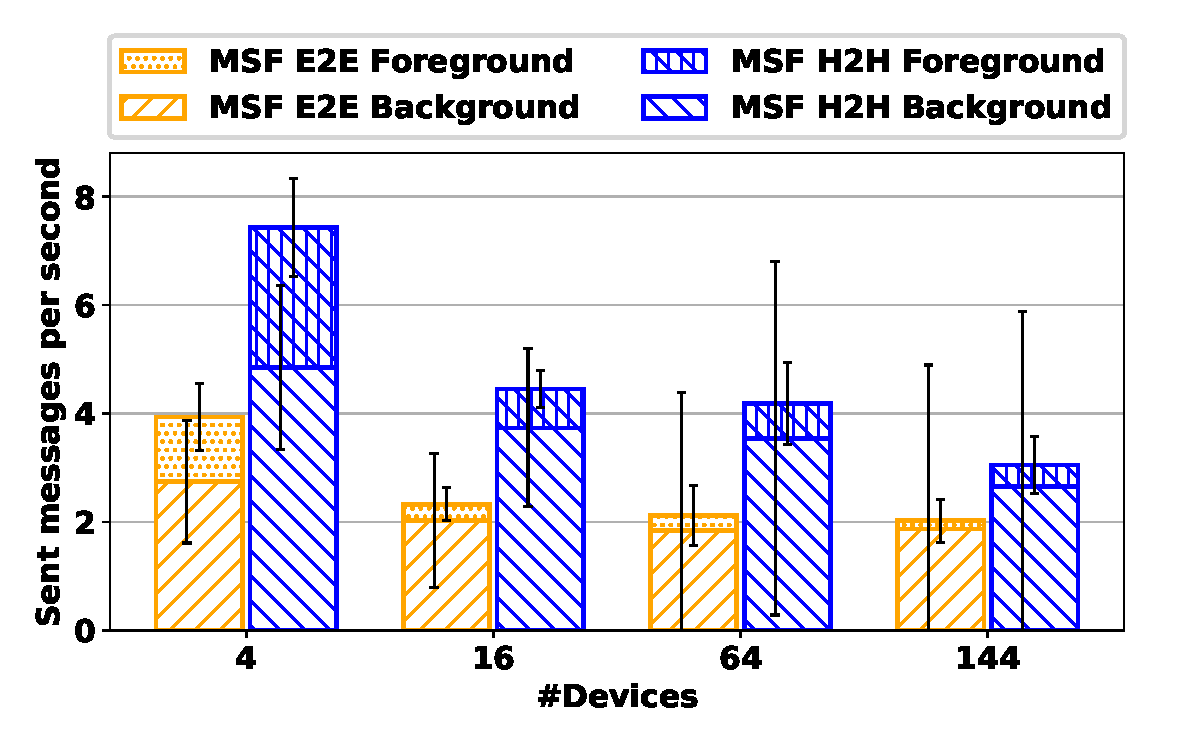
\includegraphics[width=\textwidth,alt={Stacked bar chart with error bars. x-axis: number of (virtual) devices (4, 16, 64, 144); y-axis: sent messages per second per device (0 to 8). Two stacked bars per group for the Mini \Grid{} deployment: end-to-end (orange, foreground stacked over background) and hop-to-hop (blue). Per-device bandwidth decreases as devices grow: end-to-end falls from about 4 at 4 devices to about 2 at 144, and hop-to-hop from about 7.4 to about 3, so per-device cost drops with scale.}]{CoMesh/figures/exp_eval/bandwidth_xdev_virt.pdf}
        \caption{\bf \small Deployment: Scalability of Per-(Virtual) Device Bandwidth. {\it \MSF{} = Mini \Grid. Error bars---left: background, right: foreground.}}
        \medskip
        \label{comesh:fig:bw_scale}
    \end{minipage}
    \hfill
    \begin{minipage}[b]{0.44\textwidth}
        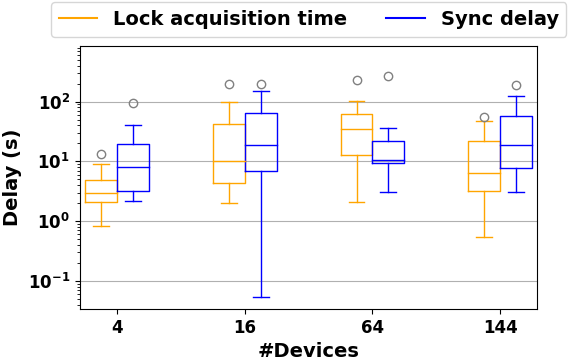
\includegraphics[width=\textwidth,alt={Grouped box-and-whisker plot. x-axis: number of devices (4, 16, 64, 144); y-axis: delay in seconds on a log scale (about 0.1 to over 100). Two series per group for the Mini \Grid{} deployment with 20 routines: lock-acquisition time (orange) and sync delay (blue). Medians range from a few seconds to about 30 seconds and stay stable as device count increases, with outliers reaching roughly 100 to 200 seconds at 64 to 144 devices.}]{CoMesh/figures/exp_eval/client_sync_delay_xdev.png}
        \caption{\bf \small Deployment: Scalability of Lock Acquisition Time and Sync Delay. {\it \MSF{} = Mini \Grid. 20 Routines.}}
        \medskip
        \label{comesh:fig:la_sync_scale}
    \end{minipage}
\end{figure}

\noindent{\bf \sysname{} Consumes Less Bandwidth than a Central Hub.} 
\Cref{comesh:fig:bw_centralized_skytali} shows decentralized \sysname's bandwidth per smart device, both  end-to-end (E2E) messages, and ad-hoc routed (hop-to-hop/H2H) messages. For fair comparison, we model a central hub over a mesh network (\Cref{comesh:section:intro}) by instantiating \sysname{} with $k=1$ and one \kgroup, i.e., a single centralized device responsible for all routines' management. We observe that: a) \sysname{} reduces bandwidth by an order of magnitude (over 10$\times$) compared to the centralized approach. b) Both end-to-end bandwidth and hop-to-hop bandwidth are scalable and remain flat, as the number of routines grows. c) Bandwidth of foreground operations (e.g.,  locking) remains small compared to background bandwidth (e.g., device monitoring). 

\noindent{\bf \sysname{} Scales with Routine Load.}
\Cref{comesh:fig:la_sync_mul_rtns} shows two per-routine metrics.  The {\it Lock Acquisition time} is the average time for a routine to acquire a device lock after it becomes available. We observe the Lock Acquisition time varies
 between 3.41 s - 13.02 s.
As the routine count increases, the median
remains stable for Mini \Grid{} (\MSF), and rises slightly for Mini \Bldg {} (\Mob) due to longer diameter and route competition.
The second metric is  {\it Sync delay}, the handover time from a finishing routine to the next already-waiting (conflicting) routine starting its first command.
We observe that with more  routines,  Sync Delay stays  stable for both \Mob{} and \MSF{},
with medians between 10.23 s - 20.833 s.

\noindent{\bf \sysname{} Scales with Number of Devices.} We scale up
by overloading each (of the 16) Pi devices as multiple ``virtual devices'' (henceforth ``nodes''). The rest of \sysname's operation remained the same. We inject 20 routines over 10 mins in the \Minigrid{} topology.  \Cref{comesh:fig:bw_scale} shows that up to 144 devices both end-to-end (E2E) and hop-wise (H2H) bandwidth {\it drop} with scale, and plateau. Background bandwidth (lower stack) plateaus quickly as the number of node \kgroups{} increases at the same rate as nodes, thus spreading load evenly.  Foreground bandwidth drops much quicker as the fixed 20 routine \kgroups{} (20) are spread over an increasing number of nodes. 

\Cref{comesh:fig:la_sync_scale} shows that both startup times for a routine---Lock Acquisition time and Sync delay---rise slowly but then plateau with scale.  Essentially, with more nodes, inter-routine conflicts become rarer.  
Median Lock Acquisition time stays in  2.97 s - 34.71 s, and  Sync Delay median is in 8.01 s - 19.04 s.

\begin{table}[tb!]
    \centering
    \caption{\bf \small \Kgroup{} Latencies in  Mini \Grid{} topology.
    }
    \bigskip
    \label{comesh:tab:kgroup_latencies}
    \tagpdfsetup{table/header-rows={1},table/header-columns={1}}
    % \tagpdfsetup{table-tagging=false}
    \footnotesize
    \begin{tabular}{c c c c}
        \hline
        \bf{\Kgroup{} delay (seconds)} & \bf{median} & \bf{mean} & \bf{q90} \\
        \hline
        Quorum reply & 1.0805 & 1.4021 & 1.4962 \\
        Leader election & 1.1675 & 1.4913 & 1.9249 \\
        State transfer & 2.0750 & 2.8468 & 3.1390 \\
        \hline
    \end{tabular}
\end{table}

\noindent{\bf \sysname{} Internal Operations are Fast.}
\Cref{comesh:tab:kgroup_latencies} shows that in \MSF{} topology on the Pis, 
\sysname's common operations are fast and take a median of 1.08 s for quorum, 1.17 s for election, and 2.08 s for state transfer during epoch change.
